\documentclass[a4paper,11pt]{article}

% ============================================================
%  Le Collé — Algèbre linéaire (compléments de deuxième année)
%  © 2026 Ahmed Amine Ouqlani
% ============================================================

% ---------- Polices ----------
\usepackage[utf8]{inputenc}
\usepackage[T1]{fontenc}
\usepackage[sc]{mathpazo}          % texte et mathématiques : Palatino
\usepackage[scaled=0.88]{helvet}   % titres et repères : linéale
\linespread{1.07}
\usepackage{amsmath,amssymb,amsthm,mathrsfs,stmaryrd}
\usepackage{microtype}

% ---------- Mise en page ----------
\usepackage[a4paper,top=2.3cm,bottom=2.3cm,left=2.4cm,right=2.4cm,
            headheight=14pt,headsep=0.8cm,footskip=1.1cm]{geometry}
\setlength{\parindent}{0pt}
\setlength{\parskip}{0.45em plus 0.15em minus 0.1em}
\raggedbottom
\emergencystretch=1.5em
\clubpenalty=10000 \widowpenalty=10000 \displaywidowpenalty=10000 \brokenpenalty=10000

% ---------- Couleurs : un bleu de nuit, un ocre, des gris ----------
\usepackage{xcolor}
\definecolor{Ink}{HTML}{1C2533}
\definecolor{Bleu}{HTML}{1F3A5F}
\definecolor{BleuMoyen}{HTML}{4A6A8F}
\definecolor{BleuClair}{HTML}{9DB2C9}
\definecolor{Fond}{HTML}{F2F4F7}
\definecolor{Ocre}{HTML}{B07A26}
\definecolor{Brique}{HTML}{A23B2A}
\definecolor{Gris}{HTML}{5E6672}
\definecolor{Filet}{HTML}{C5CCD6}

% ---------- Packages ----------
\usepackage{enumitem}
\setlist{itemsep=0.25em,topsep=0.35em,parsep=0pt}
\setlist[itemize]{label=\textcolor{BleuMoyen}{\small\textbullet},leftmargin=1.4em}
\setlist[enumerate]{leftmargin=1.8em,label=\textsf{\small\color{Bleu}\arabic*.}}
\usepackage{booktabs,array,multicol}
\usepackage{needspace,float}
\usepackage[font=small,labelfont={sf,color=Bleu},labelsep=period,skip=6pt]{caption}
\usepackage{tikz}
\usetikzlibrary{arrows.meta,calc,decorations.markings}
\usepackage{pgfplots}
\pgfplotsset{compat=1.17}
\usepackage{tkz-tab}
\usepackage[most]{tcolorbox}
\usepackage{titlesec,titletoc}
\usepackage{fancyhdr,lastpage,etoolbox}
\usepackage[colorlinks=true,linkcolor=Bleu,urlcolor=Bleu,citecolor=Bleu,
            pdftitle={DS blanc — d après Banque PT — 28 novembre 2026},pdfauthor={Ahmed Amine Ouqlani}]{hyperref}

\numberwithin{equation}{section}
\numberwithin{figure}{section}
\numberwithin{table}{section}

% ---------- Titres ----------
% numéro du chapitre dans le parcours PT (affiché), distinct de la numérotation interne
\newcommand{\grandnum}{\thesection}\newcommand{\ongletcouleur}{Bleu}
% Chapitres (sections) : grand numéro, titre en linéale, filet ocre
\titleformat{\section}[display]
  {\normalfont\sffamily\color{Ink}}
  {{\small\color{Gris}\textls[200]{\MakeUppercase{Chapitre}}}\\[-0.2em]%
   {\fontsize{64}{64}\selectfont\color{BleuClair}\grandnum}}
  {0.4em}
  {\fontsize{25}{30}\selectfont\bfseries}
  [\vspace{0.5em}{\color{Ocre}\rule{3.2cm}{1.4pt}}]
\titlespacing*{\section}{0pt}{0pt}{1.6em}
\titleformat{name=\section,numberless}[display]
  {\normalfont\sffamily\color{Ink}}{}{0pt}{\fontsize{25}{30}\selectfont\bfseries}
  [\vspace{0.5em}{\color{Ocre}\rule{3.2cm}{1.4pt}}]
\titlespacing*{name=\section,numberless}{0pt}{0pt}{1.6em}

\titleformat{\subsection}
  {\needspace{5\baselineskip}\normalfont\sffamily\Large\bfseries\color{Ink}}
  {\color{Bleu}\thesubsection}{0.8em}{}
\titlespacing*{\subsection}{0pt}{1.8em}{0.5em}
\titleformat{\subsubsection}
  {\needspace{5\baselineskip}\normalfont\sffamily\large\bfseries\color{Ink}}
  {\color{Bleu}\thesubsubsection}{0.7em}{}
\titlespacing*{\subsubsection}{0pt}{1.6em}{0.4em}
\titleformat{\paragraph}[runin]{\normalfont\sffamily\bfseries\color{Ink}}{}{0pt}{}[.]
\titlespacing*{\paragraph}{0pt}{0.9em}{0.6em}
\setcounter{secnumdepth}{3}
\setcounter{tocdepth}{2}

% ---------- Table des matières ----------
\titlecontents{section}[0pt]{\addvspace{0.7em}\sffamily\bfseries\color{Ink}}
  {}{}{\hfill\contentspage}[\addvspace{0.2em}]
\titlecontents{subsection}[2.2em]{\small\linespread{1}\selectfont}
  {\makebox[2.6em][l]{\color{Gris}\thecontentslabel}}{}{\titlerule*[0.7pc]{.}\contentspage}

% ---------- En-têtes et pieds de page ----------
\pagestyle{fancy}
\fancyhf{}
\renewcommand{\sectionmark}[1]{\markboth{#1}{}}
\fancyhead[L]{\footnotesize\sffamily\color{Gris}\leftmark}
\fancyhead[R]{\footnotesize\sffamily\scshape\color{Gris}Le Collé}
\fancyfoot[C]{\small\sffamily\color{Ink}\thepage}
\fancyfoot[L]{\scriptsize\sffamily\hyperlink{toc}{\color{Filet}sommaire}}
\renewcommand{\headrulewidth}{0.4pt}
\renewcommand{\headrule}{{\color{Filet}\hrule height\headrulewidth width\headwidth}}
\renewcommand{\footrulewidth}{0pt}
\fancypagestyle{plain}{\fancyhf{}\fancyfoot[C]{\small\sffamily\color{Ink}\thepage}\renewcommand{\headrulewidth}{0pt}}

% ---------- Énoncés ----------
\newtheoremstyle{enonce}{0pt}{0pt}{}{}{\sffamily\bfseries\color{Bleu}}{.}{0.5em}
  {\thmname{#1}\thmnumber{~#2}\thmnote{\ \normalfont\sffamily\color{Ink}(#3)}}
\newtheoremstyle{exemple}{0.9em}{0.9em}{}{}{\sffamily\bfseries\color{BleuMoyen}}{.}{0.5em}
  {\thmname{#1}\thmnumber{~#2}\thmnote{\ \normalfont\sffamily\color{Ink}(#3)}}
\newtheoremstyle{remarque}{0.7em}{0.7em}{}{}{\sffamily\itshape}{.}{0.5em}{\thmname{#1}\thmnote{\ (#3)}}
\theoremstyle{enonce}
\newtheorem{definition}{Définition}[section]
\newtheorem{theoreme}[definition]{Théorème}
\newtheorem{proposition}[definition]{Proposition}
\newtheorem{corollaire}[definition]{Corollaire}
\theoremstyle{exemple}
\newtheorem{exemple}[definition]{Exemple}
\theoremstyle{remarque}
\newtheorem*{remarque}{Remarque}

\tcbset{
  defi/.style={enhanced,breakable,colback=white,colframe=white,boxrule=0pt,arc=0pt,
     borderline west={1.2pt}{0pt}{Bleu},left=11pt,right=4pt,top=3pt,bottom=3pt,
     before skip=1.1em,after skip=1.1em},
  thm/.style={enhanced,breakable,colback=Fond,colframe=Fond,boxrule=0pt,arc=0pt,
     borderline west={2.4pt}{0pt}{Bleu},left=11pt,right=8pt,top=6pt,bottom=6pt,
     before skip=1.2em,after skip=1.2em}}
\tcolorboxenvironment{definition}{defi}
\tcolorboxenvironment{theoreme}{thm}
\tcolorboxenvironment{proposition}{thm}
\tcolorboxenvironment{corollaire}{thm}

\renewcommand{\proofname}{Démonstration}
\renewcommand{\qedsymbol}{\textcolor{BleuClair}{$\blacksquare$}}
\makeatletter
\renewenvironment{proof}[1][\proofname]{\par\pushQED{\qed}\normalfont
  \topsep0.5em\relax\trivlist\item[\hskip\labelsep\sffamily\itshape\color{Gris}#1.]\ignorespaces}
  {\popQED\endtrivlist\@endpefalse}
\makeatother

% ---------- Méthode : filets haut et bas, titre en bandeau ----------
\makeatletter\newcommand{\methlabelfix}{\protected@edef\@currentlabel{\thetcbcounter}}\makeatother
\newtcolorbox[auto counter,number within=section]{methode}[2][]{%
  enhanced,unbreakable,colback=white,colframe=white,boxrule=0pt,arc=0pt,
  borderline north={0.9pt}{0pt}{Bleu},borderline south={0.9pt}{0pt}{Bleu},
  left=4pt,right=4pt,top=8pt,bottom=8pt,before skip=1.4em,after skip=1.4em,
  before upper={\methlabelfix\phantomsection\addcontentsline{met}{metentry}{\protect\makebox[2.6em][l]{\thetcbcounter}#2}%
     {\sffamily\bfseries\small\color{white}\colorbox{Bleu}{\strut\ MÉTHODE~\thetcbcounter\ }}%
     \ \ {\sffamily\bfseries\color{Bleu}#2}\par\smallskip},#1}

% ---------- Repères pédagogiques : un filet de couleur, un mot-clé ----------
\newcommand{\definirbloc}[3]{% nom, couleur, libellé
  \newtcolorbox{#1}[1][]{enhanced,breakable,blanker,
    borderline west={1.4pt}{0pt}{#2},left=10pt,right=2pt,top=1pt,bottom=1pt,
    before skip=1em,after skip=1em,
    before upper={{\sffamily\bfseries\footnotesize\color{#2}\textls[120]{\MakeUppercase{#3}}}\quad},##1}}
\definirbloc{reflexe}{Bleu}{Réflexe}
\definirbloc{astuce}{Ocre}{Astuce}
\definirbloc{attention}{Brique}{Attention}
\definirbloc{enpratique}{BleuMoyen}{En pratique}
\definirbloc{plusloin}{Gris}{Pour aller plus loin}
\definirbloc{strategie}{Bleu}{Stratégie}
\definirbloc{lecture}{BleuMoyen}{Lire le schéma}
% compatibilité avec les parties reprises
\newenvironment{garde}{\begin{attention}}{\end{attention}}
\newenvironment{complementHP}{\begin{plusloin}}{\end{plusloin}}
\newenvironment{interpretation}{\begin{enpratique}}{\end{enpratique}}

% ---------- Exercices, corrigés ----------
\newcounter{exo}[section]
\renewcommand{\theexo}{\thesection.\arabic{exo}}
\newcommand{\niveau}[1]{{\color{Ocre}\footnotesize
  \ifcase#1\or$\bullet\circ\circ\circ\circ$\or$\bullet\bullet\circ\circ\circ$\or$\bullet\bullet\bullet\circ\circ$%
  \or$\bullet\bullet\bullet\bullet\circ$\or$\bullet\bullet\bullet\bullet\bullet$\fi}}
\newcommand{\serie}[1]{\par\needspace{8\baselineskip}\vspace{1.5em}%
  \noindent{\sffamily\bfseries\color{Bleu}#1}\par\nobreak\vspace{-0.4em}%
  \noindent{\color{Filet}\rule{\linewidth}{0.4pt}}\par\nobreak\vspace{0.1em}}
\newenvironment{exo}[3]{%
  \par\needspace{5\baselineskip}\vspace{0.75em}\refstepcounter{exo}\label{e:#1}%
  \def\exolab{#1}%
  \noindent{\sffamily\bfseries\color{Bleu}Exercice~\theexo}\quad\niveau{#2}%
  \hfill{\footnotesize\sffamily\color{Gris}#3}\par\nobreak\vspace{0.15em}}%
  {\par\nopagebreak\noindent\hfill{\scriptsize\sffamily\hyperref[c:\exolab]{\color{Gris}corrigé p.~\pageref{c:\exolab}}}\par}
\newenvironment{corrige}[1]{%
  \par\needspace{6\baselineskip}\vspace{1em}\phantomsection\label{c:#1}%
  \noindent{\sffamily\bfseries\color{Bleu}Exercice~\ref{e:#1}}\quad
  {\scriptsize\sffamily\hyperref[e:#1]{\color{Gris}énoncé p.~\pageref{e:#1}}}\par\nobreak\vspace{0.2em}}%
  {\hfill\textcolor{BleuClair}{$\square$}\par}
\newcommand{\etape}[1]{\par\smallskip\noindent{\sffamily\bfseries\small\color{BleuMoyen}#1.}\ }
\newenvironment{solution}{\par\noindent{\sffamily\bfseries\small\color{BleuMoyen}Solution.}\ }{\hfill\textcolor{BleuClair}{$\square$}\par}
\newcommand{\chercher}{\par\smallskip\noindent{\color{Filet}\rule[0.5ex]{1.2cm}{0.4pt}}\
  {\footnotesize\sffamily\itshape\color{Gris}laisser chercher l'étudiant avant de poursuivre}\par\smallskip}

% ---------- Guide de séance ----------

\newcommand{\marge}[1]{\leavevmode\marginpar{\raggedleft\scriptsize\sffamily\color{Gris}\textls[100]{\MakeUppercase{#1}}}\ignorespaces}
\newcommand{\Etape}[4]{%
  \subsection[Étape #1 --- #3 {\color{Gris}(#2)}]{#3}\label{etape:#1}%
  \noindent{\small\sffamily\color{Gris}{\color{Ocre}\bfseries Étape #1}\quad·\quad #2\quad·\quad #4}\par\medskip}
\newcommand{\question}[1]{\par\smallskip\noindent{\sffamily\bfseries\small\color{BleuMoyen}Question.}\ \textit{#1}\par\smallskip}
\newcommand{\rappel}[1]{\par\smallskip\noindent\phantomsection\addcontentsline{rap}{rapentry}{#1}%
  {\sffamily\bfseries\scriptsize\colorbox{Fond}{\color{Gris}\strut RAPPEL}}\ {\sffamily\small\color{Gris}#1.}\ }
\newcommand{\pourquoi}{\par\noindent{\sffamily\bfseries\small\color{Ocre}Pourquoi ?}\ }

% Ouverture de chapitre : \ouverture{objectifs}{prérequis}{durée}
\newcommand{\ouverture}[3]{%
  \begin{tcolorbox}[enhanced,colback=Fond,colframe=Fond,arc=0pt,boxrule=0pt,left=12pt,right=12pt,top=10pt,bottom=10pt,
     before skip=1.2em,after skip=1.6em]
  \begin{minipage}[t]{0.56\linewidth}
  {\sffamily\bfseries\small\color{Bleu}OBJECTIFS}\par\vspace{0.3em}\small #1
  \end{minipage}\hfill
  \begin{minipage}[t]{0.38\linewidth}
  {\sffamily\bfseries\small\color{Bleu}PRÉREQUIS}\par\vspace{0.3em}\small #2
  \ifx\relax#3\relax\else\par\vspace{0.6em}{\sffamily\bfseries\small\color{Bleu}DURÉE}\par\vspace{0.2em}\small #3\fi
  \end{minipage}
  \end{tcolorbox}}
% Fin de chapitre
\newenvironment{essentiel}{\par\needspace{12\baselineskip}\vspace{1.5em}%
  \begin{tcolorbox}[enhanced,unbreakable,colback=white,colframe=white,boxrule=0pt,arc=0pt,
   borderline north={1.4pt}{0pt}{Ocre},left=2pt,right=2pt,top=8pt,bottom=4pt]
  {\sffamily\bfseries\color{Ocre}L'ESSENTIEL DU CHAPITRE}\par\medskip}{\end{tcolorbox}}

% ---------- Notations ----------
\newcommand{\K}{\mathbb{K}}
\newcommand{\R}{\mathbb{R}}
\newcommand{\C}{\mathbb{C}}
\newcommand{\N}{\mathbb{N}}
\newcommand{\Z}{\mathbb{Z}}
\newcommand{\Mn}[1]{\mathcal{M}_{n}(#1)}
\newcommand{\GLn}[1]{\mathrm{GL}_n(#1)}
\newcommand{\LE}{\mathcal{L}(E)}
\newcommand{\rg}{\operatorname{rg}}
\newcommand{\vect}{\operatorname{Vect}}
\newcommand{\Mat}{\operatorname{Mat}}
\newcommand{\Id}{\operatorname{Id}}
\newcommand{\sh}{\operatorname{sh}}
\newcommand{\ch}{\operatorname{ch}}
\renewcommand{\th}{\operatorname{th}}
\DeclareMathOperator{\argsh}{argsh}
\newcommand{\vv}[1]{\overrightarrow{#1}}
\newcommand{\ve}[1]{\vec{#1}}
\newcommand{\ient}[2]{\llbracket #1,#2\rrbracket}
\newcommand{\dt}[1]{\left|\begin{matrix}#1\end{matrix}\right|}
\newcommand{\dis}{\displaystyle}

% ---------- Figures ----------
\pgfplotsset{trig format plots=rad}
\pgfplotsset{courbe/.style={axis lines=middle,axis equal image,
  axis line style={Gris,-{Stealth[length=5pt]}},
  xlabel={$x$},ylabel={$y$},ticklabel style={font=\scriptsize\sffamily,color=Gris},
  every axis x label/.style={at={(ticklabel* cs:1)},anchor=west,font=\small},
  every axis y label/.style={at={(ticklabel* cs:1)},anchor=south,font=\small},
  samples=300,smooth,width=0.6\linewidth}}
\tikzset{arcetude/.style={Bleu,line width=1.25pt},
         reste/.style={BleuClair,line width=1pt},
         tgte/.style={Ocre,line width=0.9pt},
         asy/.style={Gris,dashed,line width=0.6pt},
         pt/.style={circle,fill=Ink,inner sep=1.2pt}}

% ---------- Navigation ----------
\makeatletter
\newcommand*\l@rapentry{\@dottedtocline{1}{0em}{0em}}
\newcommand*\l@metentry{\@dottedtocline{1}{0em}{0em}}
\newcommand{\listemethodes}{\@starttoc{met}}
\newcommand{\listerappels}{\@starttoc{rap}}
\makeatother
% onglets de chapitre sur le bord droit
\usepackage{eso-pic}
\newif\ifonglets \ongletsfalse
\newcommand{\dessineronglet}{%
  \edef\ongcol{\ongletcouleur}%
  \edef\ongnum{\grandnum}%
  \pgfmathsetmacro{\ongy}{3.2+2.3*(\ongnum-1)}%
  \begin{tikzpicture}[remember picture,overlay]
  \fill[\ongcol] ([xshift=-0.75cm,yshift=-\ongy cm]current page.north east)
     rectangle ([yshift=-\ongy cm-1.9cm]current page.north east);
  \node[text=white,font=\sffamily\bfseries\large] at ([xshift=-0.37cm,yshift=-\ongy cm-0.95cm]current page.north east)
     {\ongnum};
  \end{tikzpicture}}
\AddToShipoutPictureBG{\ifonglets\ifnum\value{section}>0 \dessineronglet\fi\fi}
% blocs de navigation et d'enseignement
\definirbloc{commencer}{Gris}{Si vous commencez ici}
\definirbloc{horsprogramme}{Brique}{Hors programme}
\newcommand{\HP}{\,{\sffamily\bfseries\scriptsize\textcolor{Brique}{[HP]}}}
\newcommand{\source}[1]{{\footnotesize\sffamily\color{Gris}\,(#1)}}
\newcommand{\coupdepouce}[1]{\par\vspace{-0.2em}\noindent{\footnotesize\sffamily\color{Gris}%
  \textbf{Coup de pouce} (à donner si l'étudiant bloque) : #1}\par}
\newcommand{\pointarret}[1]{\par\vspace{1em}\noindent{\color{Filet}\rule[0.5ex]{\linewidth}{0.4pt}}\par\nobreak
  \noindent{\footnotesize\sffamily\color{Ocre}\bfseries POINT D'ARRÊT POSSIBLE}\quad{\footnotesize\sffamily\color{Gris}#1}\par\vspace{0.6em}}
\newcommand{\demarche}[1]{\noindent{\sffamily\bfseries\small\color{BleuMoyen}Démarche.}\ \textit{#1}\par\smallskip}

% ---------- Corrigés : idées, astuces, pièges, à retenir ----------
\newcommand{\choix}[1]{\par\noindent{\sffamily\bfseries\small\color{BleuMoyen}Choix de la méthode.}\ #1\par\smallskip}
\newcommand{\gain}[1]{\par\noindent{\sffamily\bfseries\small\color{Ocre}Astuce.}\ #1\par}
\newcommand{\piege}[1]{\par\noindent{\sffamily\bfseries\small\color{Brique}Piège.}\ #1\par}
\newtcolorbox{retenirbox}{enhanced,breakable,colback=Fond,colframe=Fond,arc=0pt,boxrule=0pt,
  borderline west={2pt}{0pt}{Ocre},left=8pt,right=6pt,top=4pt,bottom=4pt,before skip=0.7em,after skip=0.5em}
\newcommand{\retenir}[1]{\begin{retenirbox}{\sffamily\bfseries\footnotesize\color{Ocre}À RETENIR}\quad #1\end{retenirbox}}
\newcommand{\TD}[1]{{\color{Ocre}\bfseries TD\,#1}\ ·\ }
\newcommand{\q}[1]{\par\smallskip\noindent{\sffamily\bfseries\color{Bleu}#1}\ }
\providecommand{\iddots}{\mathinner{\mkern1mu\raise1pt\hbox{.}\mkern2mu\raise4pt\hbox{.}\mkern2mu\raise7pt\hbox{.}\mkern1mu}}


\fancyfoot[L]{}
\newcommand{\Partie}[1]{\par\needspace{5\baselineskip}\vspace{1.1em}\noindent
  {\sffamily\bfseries\large\color{Bleu}#1}\par\vspace{2pt}{\color{Filet}\rule{\linewidth}{0.4pt}}\par\smallskip}
\newcommand{\Q}[1]{\par\needspace{3\baselineskip}\medskip\noindent{\sffamily\bfseries\color{Bleu}#1}\enspace}
\setlist[enumerate,1]{label=\arabic*.,leftmargin=1.6em,itemsep=3pt,topsep=3pt}
\newcommand{\bandeau}[2]{%
\begin{tikzpicture}[remember picture,overlay]
\fill[Bleu] (current page.north west) rectangle ([yshift=-4.2cm]current page.north east);
\node[anchor=north west,text=white,font=\sffamily\footnotesize,inner sep=0] at ([xshift=2.2cm,yshift=-1.1cm]current page.north west)
  {\textls[120]{MATHÉMATIQUES · CPGE PT · DS BLANC}};
\node[anchor=north west,text=white,font=\sffamily\bfseries\LARGE,inner sep=0] at ([xshift=2.2cm,yshift=-1.75cm]current page.north west)
  {DS blanc --- d'après la Banque PT};
\node[anchor=north west,text=white,font=\sffamily\normalsize,inner sep=0] at ([xshift=2.2cm,yshift=-2.75cm]current page.north west)
  {#1};
\node[anchor=north east,text=white,font=\sffamily\scshape\large,inner sep=0] at ([xshift=-2.2cm,yshift=-1.05cm]current page.north east)
  {Le Collé};
\node[anchor=north east,text=white,font=\sffamily\small,inner sep=0] at ([xshift=-2.2cm,yshift=-2.8cm]current page.north east)
  {#2};
\end{tikzpicture}
\vspace*{2.9cm}}
\newcommand{\Source}[1]{\par\vspace{-0.3em}\noindent{\footnotesize\sffamily\color{Gris}#1}\par\smallskip}
\usetikzlibrary{patterns}\usepgfplotslibrary{fillbetween}
\fancyhead[L]{\footnotesize\sffamily\color{Gris}DS blanc · d'après la Banque PT · corrigé Le Collé}
\providecommand{\ch}{\operatorname{ch}}\providecommand{\tr}{\operatorname{tr}}\providecommand{\Sp}{\operatorname{Sp}}
\begin{document}
\pagestyle{fancy}\thispagestyle{plain}
\bandeau{Samedi 28 novembre 2026 · préparation au DS du lundi 30 novembre}{Corrigé Le Collé}

\begin{tcolorbox}[enhanced,colback=Fond,colframe=Fond,arc=0pt,boxrule=0pt,left=10pt,right=10pt,top=8pt,bottom=8pt]
\small Corrigé rédigé par Le Collé (non officiel), au niveau de rédaction attendu en devoir. Tous les résultats ont été vérifiés par
calcul formel.
\end{tcolorbox}

\Partie{Exercice 1 — Réduction de quelques matrices}

\Q{1.} Une matrice de $\mathcal M_n(\K)$ est trigonalisable dans $\mathcal M_n(\K)$ si et seulement si son polynôme caractéristique est scindé
sur $\K$. En particulier, toute matrice est trigonalisable dans $\mathcal M_n(\C)$.

\Q{2.} $\chi_{M_1}(x)=x^2-\tr(M_1)x+\det M_1=x^2-3x-4=(x-4)(x+1)$. $M_1$ est d'ordre $2$ et a deux valeurs propres réelles distinctes : elle est
\textbf{diagonalisable dans $\mathcal M_2(\R)$}, donc dans $\mathcal M_2(\C)$.
$M_1-4I_2=\begin{pmatrix}-2&6\\1&-3\end{pmatrix}$ : $E_4=\vect\big((3,1)\big)$ ; $M_1+I_2=\begin{pmatrix}3&6\\1&2\end{pmatrix}$ : $E_{-1}=\vect\big((-2,1)\big)$. Donc
\[P_1=\begin{pmatrix}3&-2\\1&1\end{pmatrix},\qquad D_1=\begin{pmatrix}4&0\\0&-1\end{pmatrix},\qquad M_1=P_1D_1P_1^{-1}.\]

\Q{3.} $\chi_{M_2}(x)=x^2-4x+5$, de discriminant $-4<0$ : les racines sont $2+i$ et $2-i$. $M_2$ n'a pas de valeur propre réelle : elle
\textbf{n'est pas diagonalisable dans $\mathcal M_2(\R)$}. Dans $\C$, elle a deux valeurs propres distinctes : elle est \textbf{diagonalisable dans
$\mathcal M_2(\C)$}. $M_2-(2+i)I_2=\begin{pmatrix}1-i&-2\\1&-1-i\end{pmatrix}$ : la deuxième ligne donne $x=(1+i)y$, d'où $E_{2+i}=\vect\big((1+i,1)\big)$ ;
la matrice étant réelle, $E_{2-i}=\vect\big((1-i,1)\big)$ (vecteur conjugué). Donc
\[P_2=\begin{pmatrix}1+i&1-i\\1&1\end{pmatrix},\qquad D_2=\begin{pmatrix}2+i&0\\0&2-i\end{pmatrix},\qquad M_2=P_2D_2P_2^{-1}.\]

\Q{4.(a)} $\chi_{M_3}(x)=x^2-6x+9=(x-3)^2$ : $\Sp(M_3)=\{3\}$. Si $M_3$ était diagonalisable, elle serait semblable à $3I_2$, donc égale à
$3I_2$ : faux. \textbf{$M_3$ n'est pas diagonalisable}. $\chi_{M_3}$ est scindé sur $\R$ : \textbf{$M_3$ est trigonalisable dans $\mathcal M_2(\R)$}.

\Q{4.(b)} On cherche $(e_1,e_2)$ avec $f_3(e_1)=3e_1$ et $f_3(e_2)=e_1+3e_2$. $M_3-3I_2=\begin{pmatrix}2&-4\\1&-2\end{pmatrix}$ : on prend $e_1=(2,1)$.
Puis $(M_3-3I_2)X=\begin{pmatrix}2\\1\end{pmatrix}$ s'écrit $x-2y=1$ : on prend $e_2=(1,0)$. $\det\begin{pmatrix}2&1\\1&0\end{pmatrix}=-1\neq0$ : $(e_1,e_2)$ est une base de
$\R^2$, et par construction la matrice de $f_3$ dans cette base est $T_3$.

\Q{5.} $\det M(a,b)=a-b$ : \textbf{$M(a,b)$ est inversible si et seulement si $a\neq b$}.

\Q{6.} $\chi(x)=x^2-(a+1)x+(a-b)$, donc $\Delta(a,b)=(a+1)^2-4(a-b)=(a-1)^2+4b$.

\Q{7.(a)} Si $\Delta(a,b)=0$, $\chi$ a une racine double $\lambda$ et $\Sp_\C(M(a,b))=\{\lambda\}$. Si $M(a,b)$ était diagonalisable dans $\mathcal M_2(\C)$,
on aurait $M(a,b)=P(\lambda I_2)P^{-1}=\lambda I_2$ ; or le coefficient $(2,1)$ de $M(a,b)$ vaut $1\neq0$. Donc $M(a,b)$ n'est pas diagonalisable dans
$\mathcal M_2(\C)$.

\Q{7.(b)} Si $\Delta(a,b)>0$, $\chi$ a deux racines réelles distinctes : $M(a,b)$ est diagonalisable dans $\mathcal M_2(\R)$ (et dans $\mathcal M_2(\C)$).
Si $\Delta(a,b)<0$, $\chi$ a deux racines complexes conjuguées distinctes, non réelles : $M(a,b)$ est diagonalisable dans $\mathcal M_2(\C)$, mais
pas dans $\mathcal M_2(\R)$ (aucune valeur propre réelle).

\Q{8.} $\Delta(a,b)=0\iff b=-\frac{(a-1)^2}4$ : c'est une parabole $\mathcal P$. Au-dessus ($\Delta>0$) : diagonalisable dans $\mathcal M_2(\R)$ ; en dessous
($\Delta<0$) : diagonalisable dans $\mathcal M_2(\C)$ seulement ; sur $\mathcal P$ : non diagonalisable. Les matrices non inversibles correspondent à la
droite $b=a$. Enfin $\Delta(2,6)=25>0$, $\Delta(3,-2)=-4<0$ et $\Delta(5,-4)=0$ : $M_1$ est au-dessus de $\mathcal P$, $M_2$ en dessous, $M_3$ sur $\mathcal P$.
\begin{center}
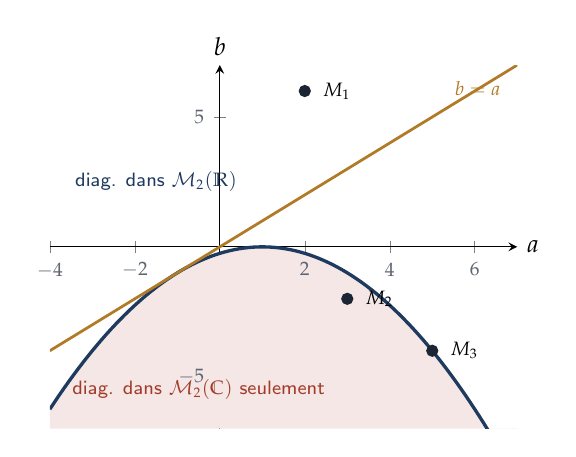
\begin{tikzpicture}
\begin{axis}[width=0.62\linewidth,height=6.2cm,axis lines=middle,xmin=-4,xmax=7,ymin=-7,ymax=7,xlabel={$a$},ylabel={$b$},
  ticklabel style={font=\scriptsize\sffamily,color=Gris},samples=100,
  every axis x label/.style={at={(ticklabel* cs:1)},anchor=west,font=\small},
  every axis y label/.style={at={(ticklabel* cs:1)},anchor=south,font=\small}]
\addplot[name path=P,Bleu,line width=1.2pt,domain=-4:7] {-(x-1)^2/4};
\path[name path=B] (axis cs:-4,-7) -- (axis cs:7,-7);
\addplot[Brique!12] fill between[of=P and B];
\addplot[Ocre,line width=1pt,domain=-4:7] {x};
\addplot[only marks,mark=*,mark size=2pt,Ink] coordinates {(2,6)(3,-2)(5,-4)};
\node[font=\scriptsize,anchor=west] at (axis cs:2.2,6) {$M_1$};
\node[font=\scriptsize,anchor=west] at (axis cs:3.2,-2) {$M_2$};
\node[font=\scriptsize,anchor=west] at (axis cs:5.2,-4) {$M_3$};
\node[font=\scriptsize\sffamily,Ocre,anchor=west] at (axis cs:5.3,6.1) {$b=a$};
\node[font=\scriptsize\sffamily,Bleu] at (axis cs:-1.5,2.5) {diag. dans $\mathcal M_2(\R)$};
\node[font=\scriptsize\sffamily,Brique] at (axis cs:-0.5,-5.5) {diag. dans $\mathcal M_2(\C)$ seulement};
\end{axis}
\end{tikzpicture}
\end{center}
{\small Parabole $\mathcal P$ (en bleu) : non diagonalisable dans $\mathcal M_2(\C)$ ; droite $b=a$ (en ocre) : non inversible.}

\Partie{Exercice 2 — Une série alternée de logarithmes}

\Q{1.} $\ln(1+h)=h-\dfrac{h^2}2+o(h^2)$ quand $h\to0$ (et même $h-\frac{h^2}2+O(h^3)$).

\Q{2.} $\frac{(-1)^n}n\to0$ et $\ln$ est continue en $1$ : $u_n\to\ln1=0$.

\Q{3.} Notons $A_N=\sum_{n\leq N}a_n$ et $B_N=\sum_{n\leq N}b_n$, qui convergent vers $A$ et $B$. Les sommes partielles de $\sum(a_n+\lambda b_n)$ sont
$A_N+\lambda B_N\to A+\lambda B$ : la série converge (et sa somme est $A+\lambda B$).

\Q{4.} Avec $h=\frac{(-1)^n}n\to0$ :
\[u_n=\frac{(-1)^n}n-\frac1{2n^2}+O\left(\frac1{n^3}\right).\]
$\sum\frac{(-1)^n}n$ converge (critère des séries alternées : $\frac1n$ décroît vers $0$), et $-\frac1{2n^2}+O\left(\frac1{n^3}\right)\sim-\frac1{2n^2}$ est de signe
constant, terme d'une série convergente (Riemann). Par la question 3, \textbf{$\sum u_n$ converge}. En revanche $|u_n|\sim\frac1n$ : \textbf{$\sum u_n$
ne converge pas absolument}.

\Q{5.(a)} Pour $p\geq1$ : $u_{2p}=\ln\frac{2p+1}{2p}$ et $u_{2p+1}=\ln\frac{2p}{2p+1}=-u_{2p}$, donc $u_{2p}+u_{2p+1}=0$. Pour $N\geq1$, on regroupe les termes
de $S_{2N}$ par paires $(2,3),(4,5),\dots,(2N-2,2N-1)$, et il reste le dernier terme :
\[S_{2N}=\sum_{p=1}^{N-1}(u_{2p}+u_{2p+1})+u_{2N}=\ln\left(\frac{2N+1}{2N}\right).\]

\Q{5.(b)} $u_{2n+1}=\ln\left(1-\frac1{2n+1}\right)=\ln\frac{2n}{2n+1}=-\ln\frac{2n+1}{2n}=-u_{2n}$.

\Q{5.(c)} Pour $N\geq2$ : $S_{2N-1}=S_{2N}-u_{2N}=\ln\frac{2N+1}{2N}-\ln\frac{2N+1}{2N}=0$.

\Q{5.(d)} $S_{2N}\to\ln1=0$ et $S_{2N-1}=0$ : les deux suites extraites de $(S_N)$ tendent vers $0$, donc $S_N\to0$.
\[\sum_{n=2}^{+\infty}\ln\left(1+\frac{(-1)^n}n\right)=0.\]

\Partie{Exercice 3 — Reste de la série exponentielle, irrationalité de $e$}

\Q{1.(a)} $R_n$ est dérivable et $R_n'(t)=e^t-\sum_{k=1}^n\frac{t^{k-1}}{(k-1)!}=e^t-\sum_{k=0}^{n-1}\frac{t^k}{k!}=R_n(t)+\frac{t^n}{n!}$. Donc $R_n'-R_n=\frac{t^n}{n!}$ :
$R_n$ est solution de $(E)$.

\Q{1.(b)} $(E_0)$ : $y'=y$. Ses solutions sur $\R$ sont $t\mapsto Ce^t$, $C\in\R$.

\Q{1.(c)} Variation de la constante : $y=C(t)e^t$ est solution si et seulement si $C'(t)e^t=\frac{t^n}{n!}$, soit $C(t)=K+\int_0^te^{-s}\frac{s^n}{n!}\,ds$.
Les solutions de $(E)$ sont $t\mapsto e^t\left(K+\displaystyle\int_0^te^{-s}\frac{s^n}{n!}\,ds\right)$, $K\in\R$.

\Q{1.(d)} $R_n(0)=1-1=0$ impose $K=0$ : pour tout $t\in\R$, $\displaystyle R_n(t)=\int_0^te^{t-s}\frac{s^n}{n!}\,ds$.

\Q{1.(e)} Si $t\geq0$ : pour $s\in[0,t]$, $0\leq e^{t-s}\frac{s^n}{n!}\leq e^t\frac{s^n}{n!}$, donc $0\leq R_n(t)\leq e^t\int_0^t\frac{s^n}{n!}\,ds=\frac{e^t\,t^{n+1}}{(n+1)!}$.
Si $t<0$ : pour $s\in[t,0]$, $t-s\leq0$, donc $\left|e^{t-s}\frac{s^n}{n!}\right|\leq\frac{|s|^n}{n!}$, et $|R_n(t)|\leq\int_t^0\frac{|s|^n}{n!}\,ds=\frac{|t|^{n+1}}{(n+1)!}$.

\Q{1.(f)} Pour $t$ fixé, $\frac{|t|^{n+1}}{(n+1)!}\to0$ (croissances comparées), donc $R_n(t)\to0$ : la série $\sum\frac{t^n}{n!}$ converge et
$e^t=\sum_{n=0}^{+\infty}\frac{t^n}{n!}$ pour tout $t\in\R$. La série entière converge en tout point : son \textbf{rayon de convergence est $+\infty$}.

\Q{2.(a)} $u_{n+1}-u_n=\frac1{(n+1)!}>0$ : $(u_n)$ est strictement croissante. Et
\begin{align*}v_{n+1}-v_n&=\frac1{(n+1)!}+\frac1{(n+1)(n+1)!}-\frac1{n\,n!}\\&=\frac{n(n+1)+n-(n+1)^2}{n(n+1)(n+1)!}=-\frac1{n(n+1)(n+1)!}<0 :\end{align*}
$(v_n)$ est strictement décroissante.

\Q{2.(b)} $v_n-u_n=\frac1{n\,n!}\to0$ : les suites sont adjacentes. Par 1.(f) avec $t=1$, $u_n\to e$ : leur limite commune est $e$.

\Q{2.(c)} Soit $q\geq1$. $(u_n)$ est strictement croissante de limite $e$ : $u_q<u_{q+1}\leq e$. $(v_n)$ est strictement décroissante de limite $e$ :
$e\leq v_{q+1}<v_q$. Donc $u_q<e<v_q$.

\Q{2.(d)} Supposons $e=\frac pq$. En multipliant par $q!>0$ : $q!\,u_q<p\,(q-1)!<q!\,u_q+\frac1q$. Or $N=q!\,u_q=\sum_{k=0}^q\frac{q!}{k!}$ est un entier, de
même que $p\,(q-1)!$. On aurait un entier strictement compris entre $N$ et $N+\frac1q\leq N+1$ : c'est impossible. Donc \textbf{$e$ est irrationnel}.

\Q{2.(e)(i)} C'est la définition de $u_n\to e$, appliquée avec $\frac\varepsilon2>0$.

\Q{2.(e)(ii)} Pour $n\geq n_0$ :
\[|w_n-e|=\left|\frac1n\sum_{k=1}^n(u_k-e)\right|\leq\frac1n\sum_{k=1}^{n_0-1}|u_k-e|+\frac1n\sum_{k=n_0}^n|u_k-e|\leq\frac Cn+\frac{n-n_0+1}n\cdot\frac\varepsilon2,\]
où $C=\sum_{k=1}^{n_0-1}|u_k-e|$ ne dépend pas de $n$. Comme $\frac Cn\to0$, il existe $n_1\geq n_0$ tel que $\frac Cn\leq\frac\varepsilon2$ pour $n\geq n_1$ ; alors
$|w_n-e|\leq\frac\varepsilon2+\frac\varepsilon2=\varepsilon$.

\Q{2.(e)(iii)} Ainsi $w_n\to e$ (lemme de Cesàro).

\Q{3.} $e_n=\exp\left(-n\ln\left(1-\frac1n\right)\right)$ et $-n\ln\left(1-\frac1n\right)=n\left(\frac1n+\frac1{2n^2}+o\left(\frac1{n^2}\right)\right)=1+\frac1{2n}+o\left(\frac1n\right)\to1$.
Par continuité de $\exp$, \textbf{$e_n\to e$}.

\Partie{Exercice 4 — Développement en série entière de la tangente}

\Q{1.(a)} Le produit de Cauchy des deux séries est $\sum c_nx^n$ avec $c_n=\sum_{k=0}^na_kb_{n-k}$. Son rayon est au moins égal au minimum des
deux rayons ; ici les deux séries convergent sur $]-R,R[$, donc le produit converge (absolument) sur $]-R,R[$, et pour $x\in\,]-R,R[$,
$\sum_{n=0}^{+\infty}c_nx^n=f(x)g(x)$.

\Q{1.(b)} Avec $g=f$ : pour tout $x\in\,]-R,R[$, $\big(f(x)\big)^2=\sum_{n=0}^{+\infty}\left(\sum_{k=0}^na_ka_{n-k}\right)x^n$.

\Q{2.(a)} Par dérivation terme à terme sur $]-R,R[$, $f'(x)=\sum_{n=0}^{+\infty}(n+1)a_{n+1}x^n$. L'égalité $f'=1+f^2$ et l'unicité du développement
en série entière donnent, pour tout $n\in\N$ :
\[(n+1)a_{n+1}=\delta_{n,0}+\sum_{k=0}^na_ka_{n-k},\qquad\text{avec }a_0=f(0)=0,\]
où $\delta_{n,0}$ vaut $1$ si $n=0$ et $0$ sinon.

\Q{2.(b)} $a_0=0$. Soit $p\geq0$ ; supposons $a_{2j}=0$ pour tout $j\leq p$. La relation avec $n=2p+1\geq1$ donne
$(2p+2)a_{2p+2}=\sum_{k=0}^{2p+1}a_ka_{2p+1-k}$. Dans chaque produit, $k$ et $2p+1-k$ sont de parités différentes : l'un est un entier pair
$\leq2p+1$, donc $\leq2p$, et le coefficient correspondant est nul. Donc $a_{2p+2}=0$. Par récurrence forte, $a_{2p}=0$ pour tout $p$.

Le développement de $f$ ne contient que des puissances impaires : pour $x\in\,]-R,R[$, $f(-x)=\sum a_{2p+1}(-x)^{2p+1}=-f(x)$ : \textbf{$f$ est impaire}.

\Q{2.(c)} $f'(0)=1+f(0)^2=1$, et $a_1=f'(0)=1$. Puis :
\begin{itemize}[leftmargin=1.2em,itemsep=2pt]
\item $n=2$ : $3a_3=a_0a_2+a_1^2+a_2a_0=1$, donc $a_3=\frac13$ ;
\item $n=4$ : $5a_5=2a_1a_3+a_2^2=\frac23$ (seuls les termes impairs comptent), donc $a_5=\frac2{15}$ ;
\item $n=6$ : $7a_7=2a_1a_5+a_3^2=\frac4{15}+\frac19=\frac{17}{45}$, donc $a_7=\frac{17}{315}$.
\end{itemize}

\Q{2.(d)} Le développement en série entière donne le développement limité (formule de Taylor-Young, $a_n=\frac{f^{(n)}(0)}{n!}$) :
\[f(x)=x+\frac{x^3}3+\frac{2x^5}{15}+\frac{17x^7}{315}+o(x^7).\]
La fonction tangente vérifie $\tan(0)=0$ et $\tan'=1+\tan^2$ sur $\left]-\frac\pi2,\frac\pi2\right[$, et elle est développable en série entière sur cet
intervalle (admis) : ses coefficients vérifient donc tout ce qui précède avec $R=\frac\pi2$. Ainsi
\[\tan x=x+\frac{x^3}3+\frac{2x^5}{15}+\frac{17x^7}{315}+o(x^7).\]
\end{document}
